\documentclass[10pt,twocolumn]{article}

\usepackage[T1]{fontenc}
\usepackage[utf8]{inputenc}
\usepackage{lmodern}
\usepackage{microtype}
\usepackage{graphicx}
\usepackage{booktabs}
\usepackage{tabularx}
\usepackage{array}
\usepackage{amsmath}
\usepackage{amssymb}
\usepackage{siunitx}
\usepackage{subcaption}
\usepackage[colorlinks=true,linkcolor=blue,citecolor=blue,urlcolor=blue]{hyperref}

\sisetup{
  round-mode=places,
  round-precision=3,
  detect-all
}

\title{\textbf{Tile-Based Quality Reconstruction for Short-Exposure Deep-Sky Imaging}\\
\large Mathematical Specification v3.3.6, Linear Reconstruction Semantics,\\
and an M31 Example Run}
\author{Jeamy Lee$^{1}$ \\ \small $^{1}$Independent Researcher / tile\_compile project}
\date{March 6, 2026}

\begin{document}
\twocolumn[
\maketitle

\begin{center}
\begin{minipage}{0.88\textwidth}
\small
\textbf{Abstract}\par
\vspace{0.35em}
Tile-Based Quality Reconstruction (TBQR) is a reconstruction methodology for short-exposure deep-sky datasets that replaces binary best-frame selection with a continuous spatio-temporal quality model. The method is defined on registered linear data and preserves the invariant that all geometrically valid frames remain contributive. Version 3.3.6 extends the earlier core with binding semantics for profile-dependent channel handling, photometrically safe overlap-add restoration, additive pre-PCC background gradient extraction (BGE), and gradient-aware photometric color calibration (PCC). This paper consolidates the mathematical definitions used by the implementation, documents the relevant functions and constraints, and grounds the method in a concrete M31 run. The example run processes 645 usable frames on a 3940x2350 canvas with 209 adaptive tiles and yields a median output FWHM of \num{4.920} px from a median seeing estimate of \num{12.346} px, corresponding to a measured improvement of \num{60.149}\%.
\end{minipage}
\end{center}

\vspace{0.35cm}
\noindent \textbf{Keywords:} astronomical image reconstruction, deep-sky imaging, short exposure stacking, robust estimation, background modeling, photometric color calibration
\vspace{0.6cm}
]

\section{Introduction}

Short-exposure deep-sky imaging intentionally acquires large numbers of comparatively noisy frames in order to average atmospheric fluctuations, tracking errors, and sensor noise over time. The classical answer to this variability is a best-frame strategy: rank frames by a global sharpness criterion, keep only the top subset, and discard the rest. This is effective in high-SNR planetary imaging, but it is a poor fit for deep-sky objects because discarded frames also discard photons, and signal-to-noise ratio scales only with the square root of retained exposure time.

TBQR replaces binary selection by a continuous weighting model. The central premise is that image quality is not a single scalar attached to the whole frame; it is the product of global atmospheric conditions and local structural fidelity. A frame may be globally noisy but still contribute usefully in tiles that remain sharp, and vice versa. The reconstruction target is therefore a per-pixel, per-tile weighted estimate assembled from all geometrically valid frames.

The current methodology version, v3.3.6, keeps the original linear reconstruction core and adds three practically important clarifications. First, channel semantics are fixed more explicitly for strict and practical profiles. Second, overlap-add reconstruction receives a recommended affine restoration step that preserves a consistent global flux scale. Third, downstream color processing is formalized: additive BGE can remove large-scale chromatic background gradients before PCC, and PCC itself may use a local plane model in the sky annulus instead of a simple constant.

\section{Invariants, Notation, and \protect \\Function Catalog}

\subsection{Binding Invariants}

The methodology is intentionally constrained by four invariants.
\begin{enumerate}
  \item \textbf{No quality-based frame selection.} Frames are not discarded because they are globally worse than other frames.
  \item \textbf{Geometric validity gating is allowed.} Frames may be rejected when registration is physically implausible, for example under reflection, catastrophic scale error, or extremely poor registration correlation.
  \item \textbf{Strict linearity in the reconstruction core.} The core uses only linear or affine operations on linear pixel values.
  \item \textbf{CFA-aware handling is preserved where relevant.} Registration and channel separation must not break Bayer phase semantics.
\end{enumerate}

These invariants separate TBQR from lucky-imaging style culling. Geometry gating suppresses failure cases; it is not a substitute ranking stage.

\subsection{Notation}

Indices and symbols follow the methodology specification:
\begin{itemize}
  \item $f$: frame index
  \item $t$: tile index
  \item $c$: channel index
  \item $p$: pixel index
  \item $I_{f,c}^{raw}(p)$: raw linear input frame
  \item $I_{f,c}(p)$: globally normalized frame
  \item $B_{f,c}$: global background estimate
  \item $\sigma_{f,c}$: global noise estimate on normalized data
  \item $E_{f,c}$: global gradient energy on normalized data
  \item $Q_{f,c}$: global quality index
  \item $G_{f,c}$: global weight
  \item $Q_{f,t,c}^{local}$: local tile quality index
  \item $L_{f,t,c}$: local tile weight
  \item $W_{f,t,c}$: effective reconstruction weight
  \item $R_{t,c}(p)$: reconstructed tile
\end{itemize}

\begin{table*}[t]
\centering
\caption{Core mathematical functions used by TBQR v3.3.6.}
\begin{tabularx}{\textwidth}{>{\raggedright\arraybackslash}p{0.17\textwidth} >{\raggedright\arraybackslash}p{0.31\textwidth} X}
\toprule
\textbf{Name} & \textbf{Definition} & \textbf{Role} \\
\midrule
Robust z-score &
$z(x_i)=\dfrac{x_i-\operatorname{median}(x)}{\max(1.4826\operatorname{MAD}(x),\varepsilon_{mad})}$ &
Robust metric normalization for background, noise, gradient energy, FWHM, contrast, and related sequences. \\
\addlinespace
Clip &
$\operatorname{clip}(x,a,b)=\min(\max(x,a),b)$ &
Bounds quality indices and geometry parameters to numerically stable ranges. \\
\addlinespace
Global weight &
$G_{f,c}=\exp(k_{global}\operatorname{clip}(Q_{f,c},-3,+3))$ &
Maps robust global quality to a strictly positive atmospheric weight. \\
\addlinespace
Local weight &
$L_{f,t,c}=\exp(\operatorname{clip}(Q_{f,t,c}^{local},-3,+3))$ &
Maps local tile quality to a strictly positive structural weight. \\
\addlinespace
Effective weight &
$W_{f,t,c}=G_{f,c}L_{f,t,c}$ &
Combines global and local quality multiplicatively. \\
\addlinespace
Hann window &
$h(i,N)=0.5\!\left(1-\cos\!\left(\dfrac{2\pi i}{N-1}\right)\right)$ &
Separable overlap-add blending function used to suppress tile seams. \\
\addlinespace
Huber loss &
$\rho(r)=\frac{1}{2}r^2$ for $|r|\le \delta$, else $\delta(|r|-\frac{1}{2}\delta)$ &
Robust loss for BGE surface fitting and related stable regression tasks. \\
\addlinespace
Cluster weight &
$w_k=\exp(\kappa_{cluster}Q_k)$ &
Optional quality-weighted aggregation of synthetic cluster outputs. \\
\bottomrule
\end{tabularx}
\label{tab:functions}
\end{table*}

\section{Core Reconstruction \protect \\Mathematics}

\subsection{Global Linear Normalization}

The core starts from linear, registered input data. For each frame and channel,
\begin{equation}
  B_{f,c} = \operatorname{median}(I_{f,c}^{raw}),
\end{equation}
\begin{equation}
  I_{f,c}(p) = \frac{I_{f,c}^{raw}(p)}{\max(B_{f,c}, \varepsilon_{bg})},
\end{equation}
with recommended default $\varepsilon_{bg}=10^{-6}$. Noise $\sigma_{f,c}$ and gradient energy $E_{f,c}$ are measured only after this linear normalization. No nonlinear tone curve is permitted in the core reconstruction path.

\subsection{Global Quality Index and \protect \\Adaptive Weights}

The global quality index is defined as
\begin{equation}
  Q_{f,c} =
  \alpha\bigl(-z(B_{f,c})\bigr) +
  \beta\bigl(-z(\sigma_{f,c})\bigr) +
  \gamma z(E_{f,c}),
\end{equation}
subject to
\begin{equation}
  \alpha + \beta + \gamma = 1.
\end{equation}
Default static weights are $(\alpha,\beta,\gamma)=(0.4,0.3,0.3)$ in the normative method. The example M31 run uses an adaptive variant with configured nominal weights $(0.40, 0.35, 0.25)$ and exponent scale $k_{global}=1.2$.

For numerical stability the score is clamped before exponentiation:
\begin{equation}
  Q_{f,c}^{clamped} = \operatorname{clip}(Q_{f,c}, -3, +3),
\end{equation}
\begin{equation}
  G_{f,c} = \exp(k_{global} Q_{f,c}^{clamped}).
\end{equation}
If adaptive global weighting is enabled, metric variances are evaluated on their robustly normalized sequences, clipped to a conservative interval, and re-normalized to sum to one. This keeps the weighting responsive without allowing a single unstable metric to dominate.

\subsection{Adaptive Tile Geometry}

Tile size is tied to the robust seeing estimate $F$ (FWHM in pixels). With image dimensions $W,H$, size factor $s$, minimum size $T_{min}$, overlap fraction $o$, and divisor bound $D$,
\begin{equation}
  T_0 = sF,
\end{equation}
\begin{equation}
  T = \left\lfloor \operatorname{clip}\!\left(T_0, T_{min}, \left\lfloor \frac{\min(W,H)}{D} \right\rfloor \right) \right\rfloor,
\end{equation}
\begin{equation}
  O = \lfloor \operatorname{clip}(o,0,0.5) \cdot T \rfloor,
  \qquad
  S = T - O.
\end{equation}
Guards ensure $F>0$, $T_{min}\ge 16$, and $S>0$ after a deterministic fallback.

Tiles are then classified using local source content:
\begin{itemize}
  \item \textbf{STAR tile}: $\operatorname{star\_count} \ge \texttt{tile.star\_min\_count}$
  \item \textbf{STRUCTURE tile}: otherwise
\end{itemize}
This classification lets the local quality model adapt to stellar fields versus extended diffuse structure.

\subsection{Local Tile Metrics and \protect \\Effective Weights}

For STAR tiles the local score is
\begin{equation}
\begin{aligned}
  Q_{f,t,c}^{star}
  &=
  0.6\bigl(-z(\mathrm{FWHM}_{f,t,c})\bigr) \\
  &\quad + 0.2z(R_{f,t,c})
  + 0.2z(C_{f,t,c}),
\end{aligned}
\end{equation}
where $R_{f,t,c}$ is roundness and $C_{f,t,c}$ is local contrast. For STRUCTURE tiles,
\begin{equation}
  Q_{f,t,c}^{struct}
  =
  0.7z((E/\sigma)_{f,t,c})
  - 0.3z(B_{f,t,c}).
\end{equation}
After clamping,
\begin{equation}
  Q_{f,t,c}^{local} = \operatorname{clip}(Q_{f,t,c}^{star|struct}, -3, +3),
\end{equation}
\begin{equation}
  L_{f,t,c} = \exp(Q_{f,t,c}^{local}),
\end{equation}
and the effective weight becomes
\begin{equation}
  W_{f,t,c} = G_{f,c}L_{f,t,c}.
\end{equation}
This factorization is important: global atmospheric quality and local structural fidelity are modeled independently and only combined at the end.

\subsection{Tile Reconstruction and \protect \\Overlap-Add}

For each tile $t$, channel $c$, and pixel $p$ inside the tile support,
\begin{equation}
  D_{t,c} = \sum_f W_{f,t,c}.
\end{equation}
If $D_{t,c}\ge \varepsilon_{weight}$,
\begin{equation}
  R_{t,c}(p) = \frac{\sum_f W_{f,t,c} I_{f,c}(p)}{D_{t,c}},
\end{equation}
else the method falls back to the unweighted arithmetic mean,
\begin{equation}
  R_{t,c}(p) = \frac{1}{N}\sum_f I_{f,c}(p),
\end{equation}
with fallback state recorded in diagnostics.

Before overlap-add, each reconstructed tile is normalized by a robust affine transform:
\begin{equation}
  bg_t = \operatorname{median}(R_{t,c}),
  \qquad
  X_t = R_{t,c} - bg_t,
\end{equation}
\begin{equation}
  m_t = \operatorname{median}(|X_t|).
\end{equation}
\begin{equation}
  Y_t =
  \begin{cases}
    X_t/m_t, & m_t \ge \varepsilon_{median} \\
    X_t, & \text{otherwise}.
  \end{cases}
\end{equation}
Tiles are blended with the separable two-dimensional Hann window
\begin{equation}
  w(x,y)=h(x,W_t)h(y,H_t),
\end{equation}
using accumulators
\begin{equation}
  A \leftarrow A + wY_t,
  \qquad
  S \leftarrow S + w,
\end{equation}
followed by
\begin{equation}
  I_{rec} = \frac{A}{\max(S,\varepsilon_{weight})}.
\end{equation}

Version 3.3.6 adds an explicit photometric restoration step. Let
\begin{equation}
  m_{global} = \operatorname{median}_t(m_t),
  \qquad
  bg_{global} = \operatorname{median}_t(bg_t).
\end{equation}
Then the globally restored image is
\begin{equation}
  I_{final} = I_{rec}m_{global} + bg_{global}.
\end{equation}
This preserves a consistent affine photometric scale while keeping the overlap-add stage itself numerically well conditioned.

\subsection{Clustering and Synthetic Frames}

When the dataset is sufficiently large, TBQR can represent atmospheric states explicitly by clustering frame descriptors. The state vector is
\begin{equation}
  v_f =
  \Bigl(
  G_{f,*},
  \operatorname{mean}_t(Q_{f,t,*}^{local}),
  \operatorname{var}_t(Q_{f,t,*}^{local}),
  B_{f,*},
  \sigma_{f,*}
  \Bigr).
\end{equation}
The number of clusters is bounded by
\begin{equation}
  K = \operatorname{clip}\!\left(\left\lfloor \frac{N}{10} \right\rfloor, K_{min}, K_{max}\right).
\end{equation}

For cluster $k$, a synthetic frame may be formed globally,
\begin{equation}
  S_{k,c} = \frac{\sum_{f \in k} G_{f,c}I_{f,c}}{\sum_{f \in k} G_{f,c}},
\end{equation}
or by a tile-weighted construction using the same $W_{f,t,c}$ logic as the core. In the full normative method, cluster outputs may be aggregated by
\begin{equation}
  Q_k = \operatorname{median}_{f \in k}(Q_{f,c}^{clamped}),
\end{equation}
\begin{equation}
  w_k = \exp(\kappa_{cluster}Q_k),
\end{equation}
\begin{equation}
  R_c = \frac{\sum_k w_kS_{k,c}}{\sum_k w_k},
\end{equation}
optionally capped by $w_k \leftarrow \min(w_k, r_{cap}\operatorname{median}_j(w_j))$. The M31 example run uses tile-weighted synthetic frames with 12 clusters but leaves optional cluster-quality weighting disabled in configuration.

\section{Downstream Linear \protect \\Post-Processing}

\subsection{Pre-PCC Background Gradient Extraction}

BGE is an additive extension applied after reconstruction and before PCC:
\begin{equation}
  I'_c(x,y) = I_c(x,y) - B_c(x,y).
\end{equation}
Only additive correction is allowed; multiplicative shading correction is explicitly forbidden in this stage.

TBQR reuses the reconstruction tiles as background sampling units. After excluding stars, strong local structure, saturated pixels, and optional object masks, each tile yields a robust background sample
\begin{equation}
  b_{t,c} = \operatorname{quantile}_q(R_{t,c}[M_{bg}]),
\end{equation}
with configurable $q \in (0,0.5]$. Optional reliability weights are defined as
\begin{equation}
  w_t =
  \exp(-\lambda \, \mathrm{structure\_score}_t)
  \bigl(1-\mathrm{masked\_fraction}_t\bigr).
\end{equation}

To suppress overfitting, tile samples are aggregated into a coarser grid. With spacing $G$,
\begin{equation}
  \mathrm{cell}_x = \left\lfloor \frac{x_t}{G} \right\rfloor,
  \qquad
  \mathrm{cell}_y = \left\lfloor \frac{y_t}{G} \right\rfloor.
\end{equation}
Per-cell values are aggregated robustly:
\begin{equation}
  b_{cell} = \operatorname{median}\{b_{t,c}\},
  \qquad
  w_{cell} = \operatorname{median}\{w_t\}.
\end{equation}
If a cell has fewer than $\texttt{bge.min\_tiles\_per\_cell}$ contributors, a deterministic fill or expansion strategy is required.

The binding polynomial surface model is
\begin{equation}
  B_c(x,y) = \sum_{m+n \le d} a_{mn}x^my^n,
\end{equation}
with coefficients obtained by robust minimization
\begin{equation}
  \arg\min_a \sum_i w_i \rho\!\left(b_i - B_c(x_i,y_i)\right),
\end{equation}
where $\rho$ is typically Huber or Tukey loss, solved by IRLS or an equivalent deterministic method. Thin-plate splines, bicubic splines, or regularized RBF surfaces are permissible alternatives if the resulting model remains large-scale and smooth.

When auto-tuning is enabled, candidate BGE configurations are scored by
\begin{equation}
  J = E_{cv} + \alpha E_{flat} + \beta E_{rough},
\end{equation}
where $E_{cv}$ is deterministic holdout residual RMS, $E_{flat}$ measures large-scale background energy, and $E_{rough}$ penalizes second-derivative waviness. The coarse grid spacing itself is defined by
\begin{equation}
  G = \operatorname{clip}\!\left(\max\!\left(2T,\frac{\min(W,H)}{N_g}\right), G_{min}, G_{max}\right),
\end{equation}
ensuring the background model is always coarser than the reconstruction tiles.

\subsection{Photometric Color Calibration}

PCC operates on linear RGB output. Version 3.3.6 formalizes a gradient-aware local background model in the sky annulus. Besides the legacy constant-median option, the annulus may fit a local plane
\begin{equation}
  bg(\Delta x,\Delta y) = a + b\Delta x + c\Delta y.
\end{equation}
If the plane fit fails, the implementation must fall back deterministically to the median model.

When a seeing estimate is available, PCC radii may be chosen automatically:
\begin{equation}
  r_{ap} = \max(r_{min}, m_{ap} \cdot \mathrm{FWHM}),
\end{equation}
\begin{equation}
  r_{in} = \max(r_{ap}+1, m_{in} \cdot \mathrm{FWHM}),
\end{equation}
\begin{equation}
  r_{out} = \max(r_{in}+2, m_{out} \cdot \mathrm{FWHM}).
\end{equation}
The example run uses $\texttt{pcc.background\_model=plane}$ and $\texttt{pcc.radii\_mode=auto\_fwhm}$ with multipliers $(1.8, 3.0, 5.0)$.

\section{M31 Example Run}

\subsection{Dataset and Operative \protect \\Configuration}

This section summarizes an example run based on M31.
The dataset is processed on a 3940x2350 canvas with 645 usable frames, an exposure time of 10 s per frame, and a common overlap fraction of \num{0.963}.
The adaptive tile geometry produces 209 tiles of size \SI{296}{px} with stride \SI{208}{px} and overlap \SI{88}{px}.
Reduced-mode clustering is not used because the frame count is well above the full-mode threshold.

\begin{table}[t]
\centering
\caption{Key configuration and dataset facts for the M31 example run.}
\begin{tabular}{ll}
\toprule
\textbf{Quantity} & \textbf{Value} \\
\midrule
Usable frames & 645 \\
Exposure time per frame & 10 s \\
Canvas size & \num{3940}x\num{2350} px \\
Common overlap fraction & 0.9630 \\
Tiles & 209 \\
Tile size / stride & 296 px / 208 px \\
Median seeing FWHM & 12.3455 px \\
Synthetic frame mode & tile\_weighted \\
Synthetic states & 12 clusters \\
Cluster size range & 27 to 102 frames \\
BGE autotune & conservative \\
PCC background model & plane \\
PCC radii mode & auto\_fwhm \\
\bottomrule
\end{tabular}
\label{tab:m31_config}
\end{table}

\begin{figure*}[t]
  \centering
  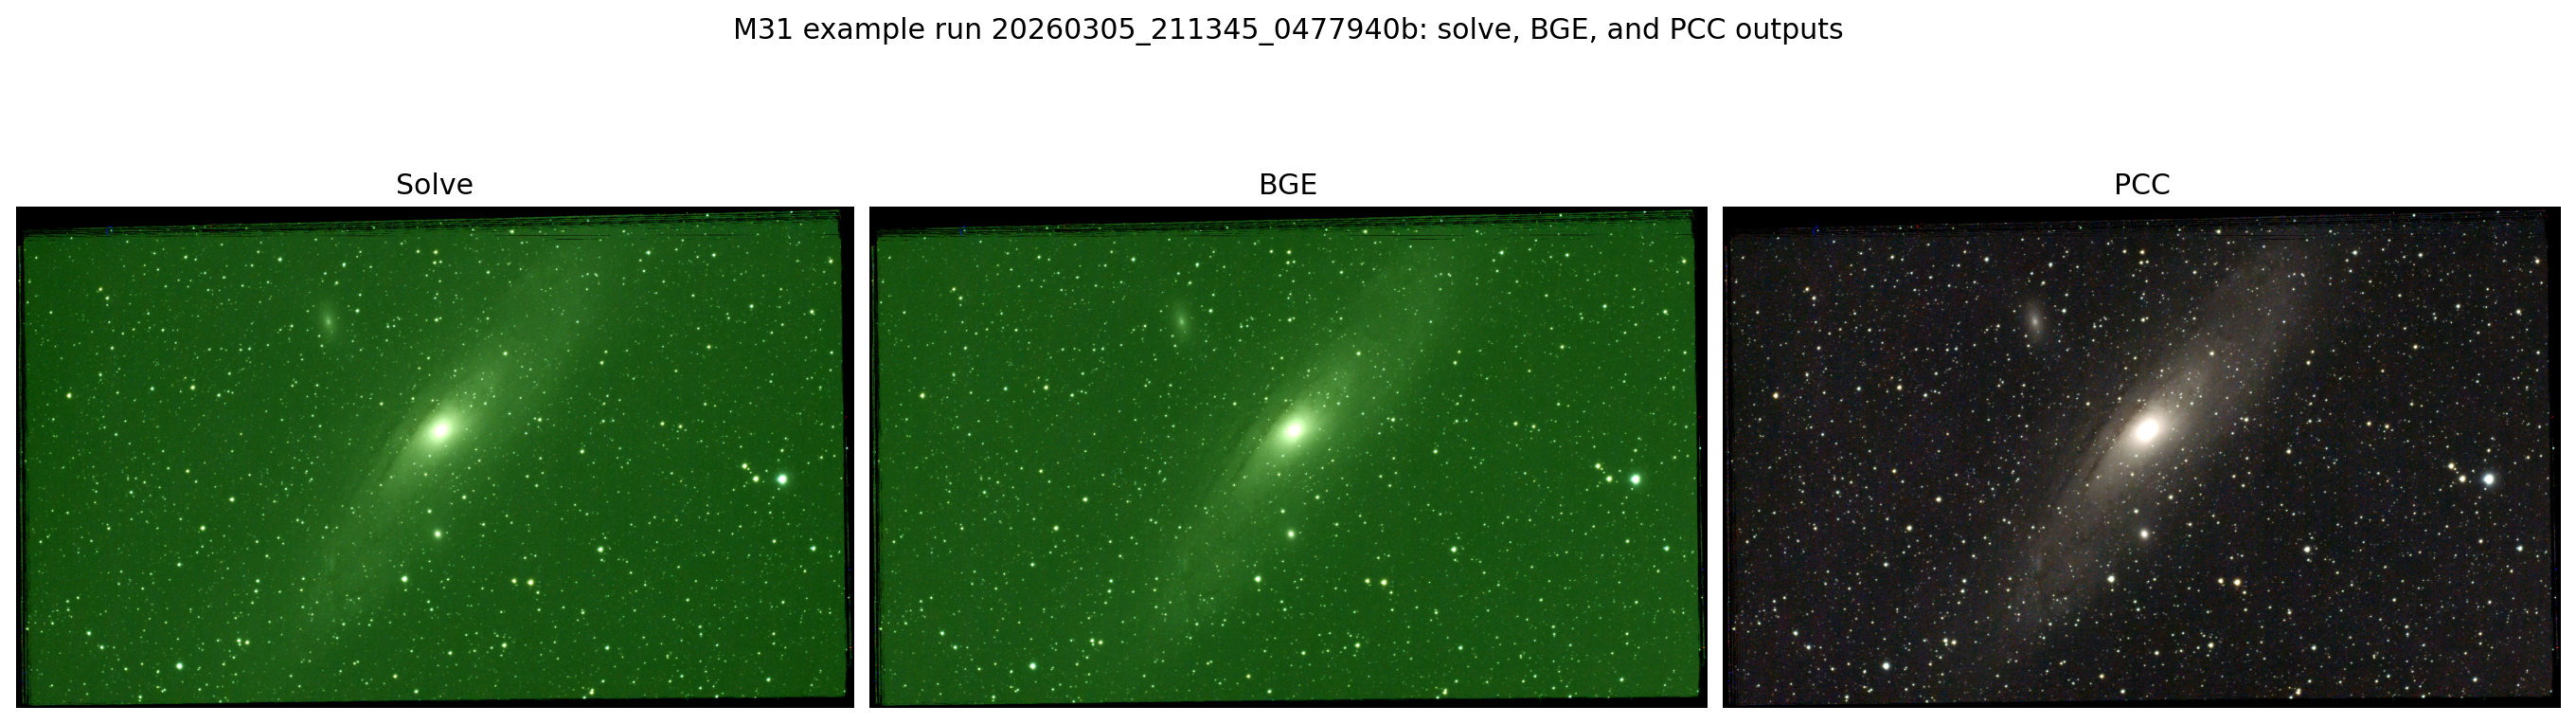
\includegraphics[width=\textwidth]{m31_stage_comparison.png}
  \caption{Example RGB outputs from the M31 run. The left panel shows the astrometrically solved linear RGB stack, the middle panel the additive BGE stage, and the right panel the final PCC-calibrated output. Display stretch is a shared asinh mapping for visualization only and is not part of the linear reconstruction core.}
  \label{fig:m31_stage}
\end{figure*}

\begin{figure}[t]
  \centering
  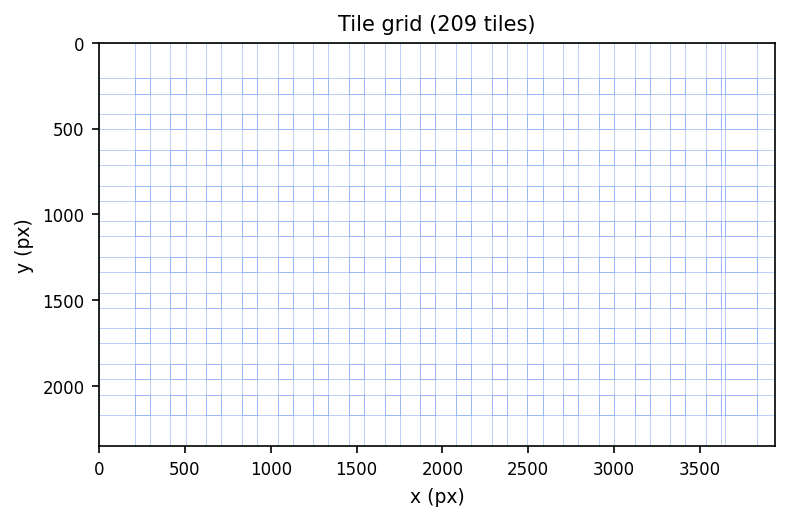
\includegraphics[width=\columnwidth]{tile_grid_overlay.png}
  \caption{Adaptive reconstruction tile grid for the M31 example run. The grid follows the seeing-driven tile size computed from the v3.3.6 geometry rules.}
  \label{fig:tile_grid}
\end{figure}

\subsection{Diagnostics and Measured \protect \\Outcomes}

Global metrics confirm that the sequence contains measurable atmospheric variation rather than a constant-quality time series. Over 645 frames, the per-frame median values are: FWHM \num{9.503} px, weighted FWHM \num{10.022} px, noise \num{0.0200}, gradient energy \num{0.00686}, background \num{208.5}, and global weight \num{0.989}; the global weight reaches a maximum of \num{3.121}. Registration correlation spans a wide range with median \num{0.575}, which justifies explicit geometric validity gating before quality-weighted accumulation.

\begin{figure}[t]
  \centering
  \begin{subfigure}[t]{\columnwidth}
    \centering
    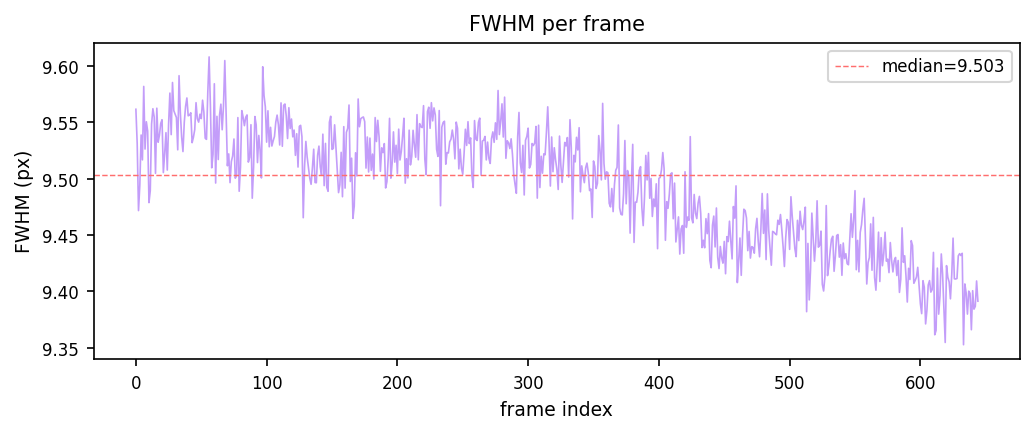
\includegraphics[width=\linewidth]{global_fwhm.png}
    \caption{Global FWHM over the frame sequence.}
  \end{subfigure}

  \vspace{0.4em}

  \begin{subfigure}[t]{\columnwidth}
    \centering
    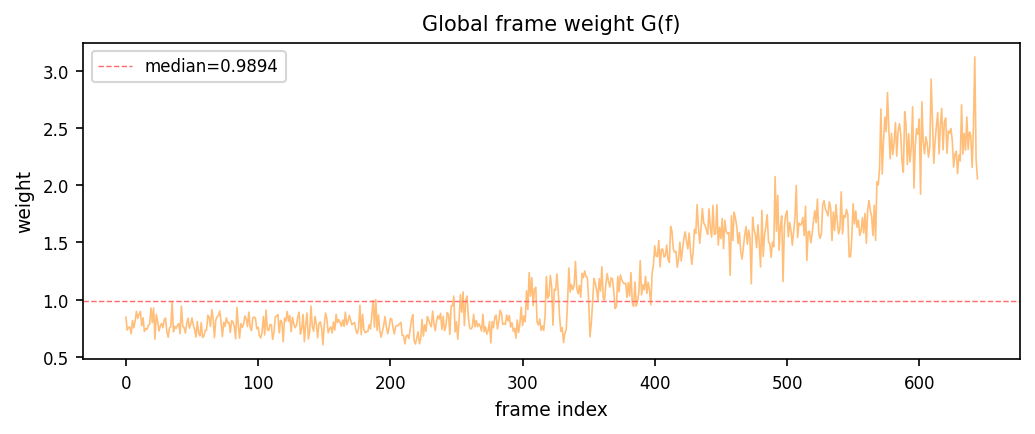
\includegraphics[width=\linewidth]{global_weight_timeseries.png}
    \caption{Adaptive global weights over time.}
  \end{subfigure}
  \caption{Global diagnostics from the M31 run.}
  \label{fig:global_diagnostics}
\end{figure}

\begin{figure*}[t]
  \centering
  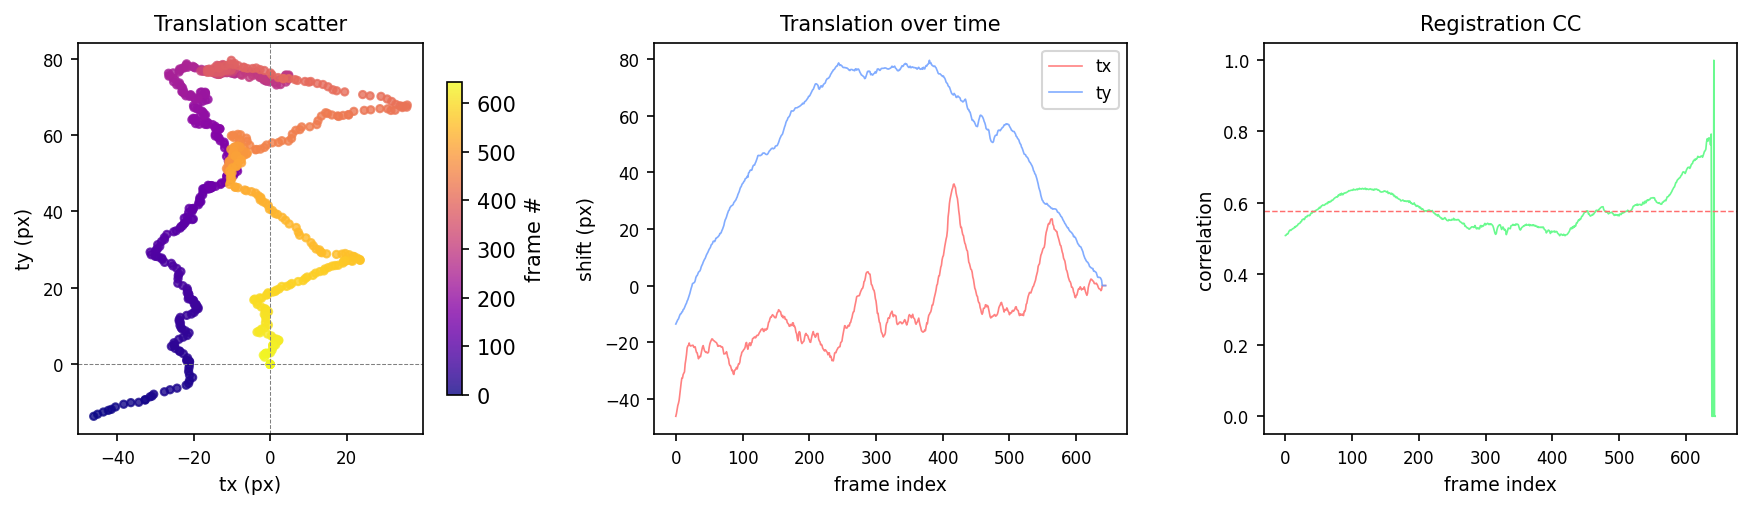
\includegraphics[width=\textwidth]{registration_overview.png}
  \caption{Registration diagnostics across the M31 run. The method uses these quantities only for validity gating, not for best-frame ranking.}
  \label{fig:registration}
\end{figure*}

\begin{figure*}[t]
  \centering
  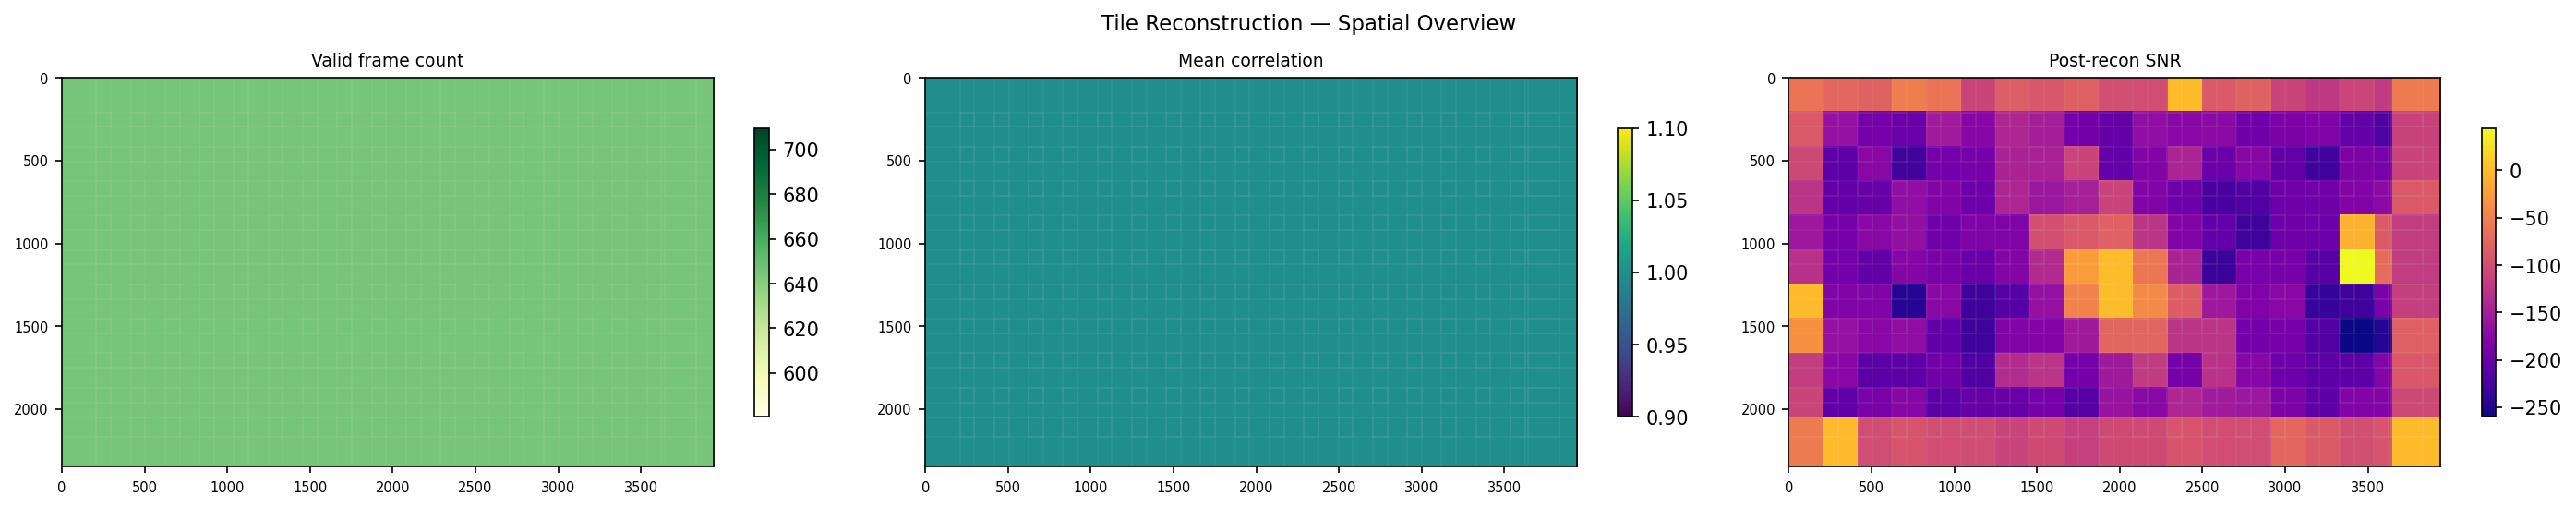
\includegraphics[width=\textwidth]{recon_spatial_overview.png}
  \caption{Spatial reconstruction diagnostics. Coverage, local SNR, local contrast, and related maps show why a tile-wise model is required instead of a single frame-level quality score.}
  \label{fig:recon_overview}
\end{figure*}

The tile reconstruction artifacts indicate stable behavior. No tile fallback was used in any of the 209 tiles, and the validation report records tile-weight variance \num{0.1860}, tile-pattern ratio p95 \num{1.0358}, and tile-pattern status `ok'. The final validation metrics are stronger than the minimum criteria: median output FWHM is \num{4.9198} px versus a median seeing estimate of \num{12.3455} px, corresponding to a measured improvement of \num{60.149}\%.

\begin{figure}[t]
  \centering
  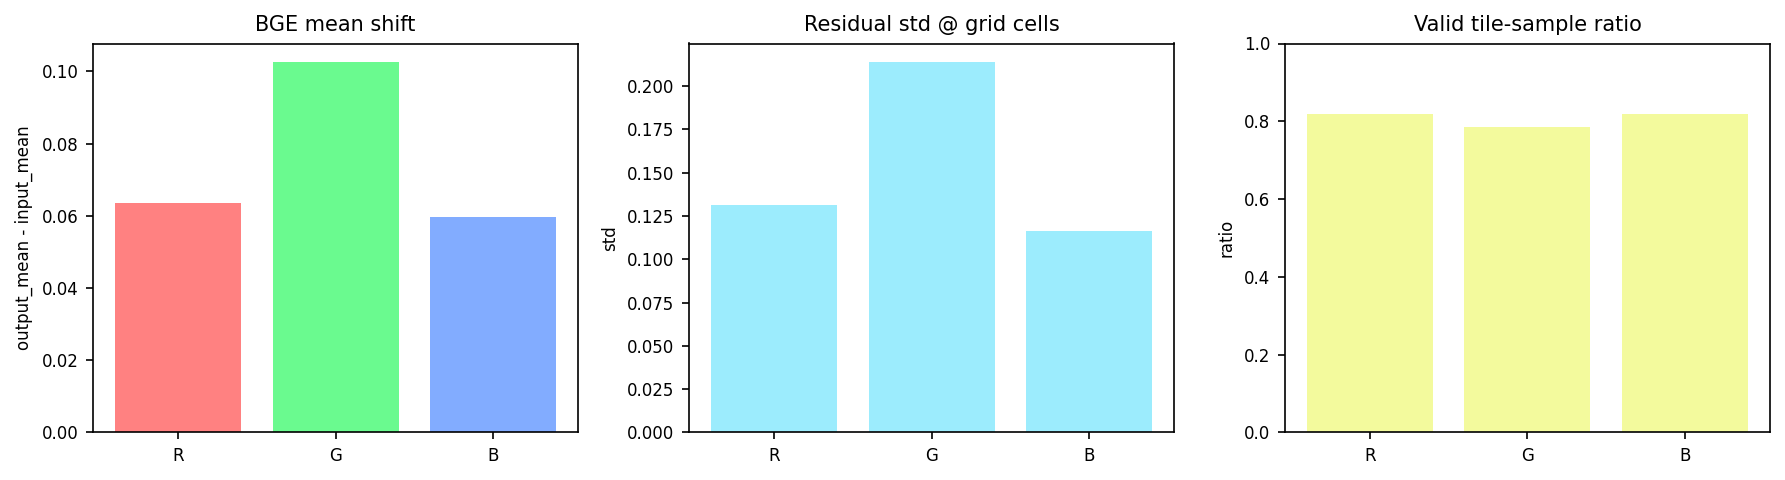
\includegraphics[width=\columnwidth]{bge_channel_summary.png}
  \caption{Per-channel BGE diagnostics. The auto-tuned run selected a polynomial surface family and applied BGE in all RGB channels.}
  \label{fig:bge}
\end{figure}

For the downstream color path, BGE was enabled with conservative autotuning and selected a polynomial fit family with sample quantile \num{0.10} and structure-threshold percentile \num{0.85}. Each color channel used 28 valid coarse-grid cells; the fit RMS residuals were \num{0.1319} (R), \num{0.2146} (G), and \num{0.1171} (B). PCC then operated with a local plane background model and auto-FWHM aperture scaling.

\begin{table}[t]
\centering
\caption{Selected quantitative outcomes from the M31 example run.}
\begin{tabular}{lr}
\toprule
\textbf{Metric} & \textbf{Value} \\
\midrule
Median seeing FWHM & 12.3455 px \\
Median output FWHM & 4.9198 px \\
FWHM improvement & 60.1489\% \\
Tile fallback count & 0 / 209 \\
Tile weight variance & 0.1860 \\
Tile-pattern ratio p95 & 1.0358 \\
Registration CC median & 0.5754 \\
Global weight median / max & 0.9894 / 3.1208 \\
BGE fit RMS (R/G/B) & 0.1319 / 0.2146 / 0.1171 \\
\bottomrule
\end{tabular}
\label{tab:m31_results}
\end{table}

\begin{figure}[t]
  \centering
  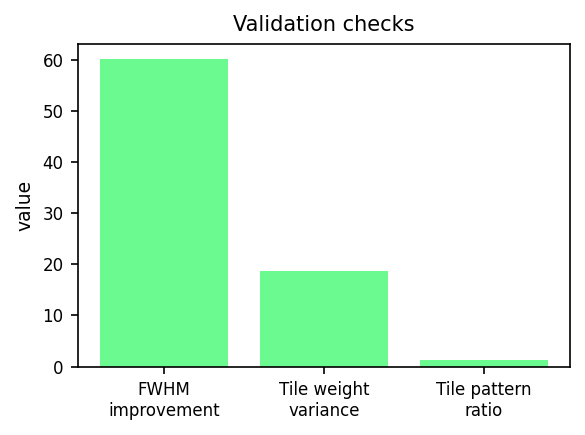
\includegraphics[width=\columnwidth]{validation_summary.png}
  \caption{Validation summary for the M31 run. The measured outputs satisfy the v3.3.6 success criteria represented in the report artifacts.}
  \label{fig:validation}
\end{figure}

\subsection{Interpretation}

The M31 run illustrates the central argument of TBQR. Atmospheric and structural quality vary significantly, but these fluctuations are not spatially uniform and therefore cannot be handled optimally with a single keep-or-discard decision. The tile-wise model absorbs this variability without downstream quality culling. At the same time, the additive BGE and gradient-aware PCC stages show that color calibration stability depends not only on the reconstruction core, but also on the treatment of large-scale channel-dependent backgrounds.

\section{Discussion}

From a methodological point of view, the most important property of TBQR is separation of concerns. Registration validity gating protects the reconstruction from geometric nonsense. Global weights model frame-level atmosphere and transparency. Local weights model tile-level sharpness and structure. Overlap-add then fuses these local estimates into a globally smooth image. BGE and PCC are explicitly downstream so that color calibration cannot silently perturb core weights.

The main practical limitation is computational scale. A full run may contain hundreds of frames, hundreds of tiles, and several downstream model-selection branches. This is why v3.3.6 defines conservative clamps, deterministic fallbacks, and explicit diagnostics. The example run shows that those constraints are not cosmetic; they are necessary for making the method numerically auditable.

\section{Conclusion}

TBQR v3.3.6 provides a mathematically explicit alternative to best-frame deep-sky stacking. Its defining semantics are simple: keep all geometrically valid frames, preserve linearity, and let quality enter as a continuous spatio-temporal weight rather than a binary acceptance flag. The methodology is sufficiently rich to include state clustering, affine-safe overlap-add restoration, additive gradient extraction, and gradient-aware PCC, while still remaining deterministic and diagnosable. The M31 example run shows that these constraints are not merely formal; they remain operational on a real short-exposure deep-sky dataset.

\noindent
The public project repository provides the implementation sources, the normative methodology and process documentation, example configurations, and experimental binary releases:
\url{https://github.com/jeamy/tile_compile}

\section*{Additional Statistical Diagnostics}

\noindent
The following diagnostic overview consolidates the most relevant run statistics in a compact closing summary. It complements the main text with background, noise, structure, registration, and frame-flow summaries from the M31 example run.

\begin{figure*}[!t]
  \centering
  \begin{subfigure}[t]{0.31\textwidth}
    \centering
    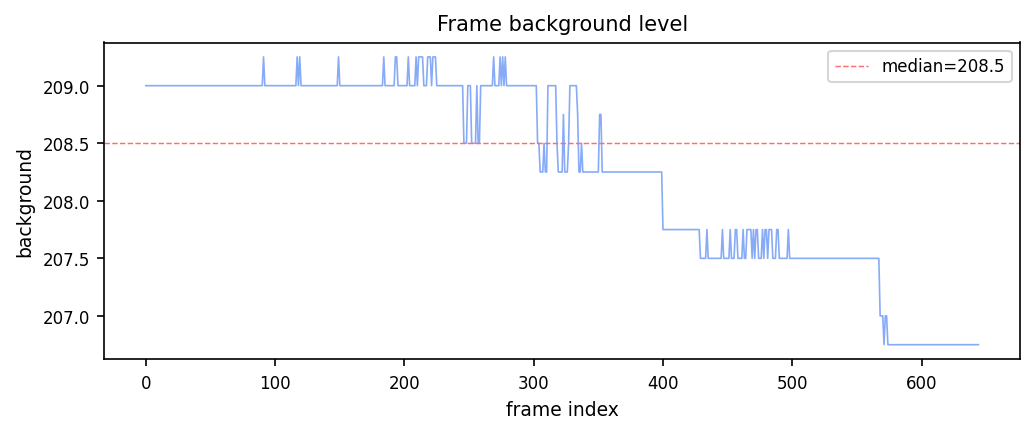
\includegraphics[width=\linewidth]{global_background.png}
    \caption{Global background trajectory.}
  \end{subfigure}
  \hfill
  \begin{subfigure}[t]{0.31\textwidth}
    \centering
    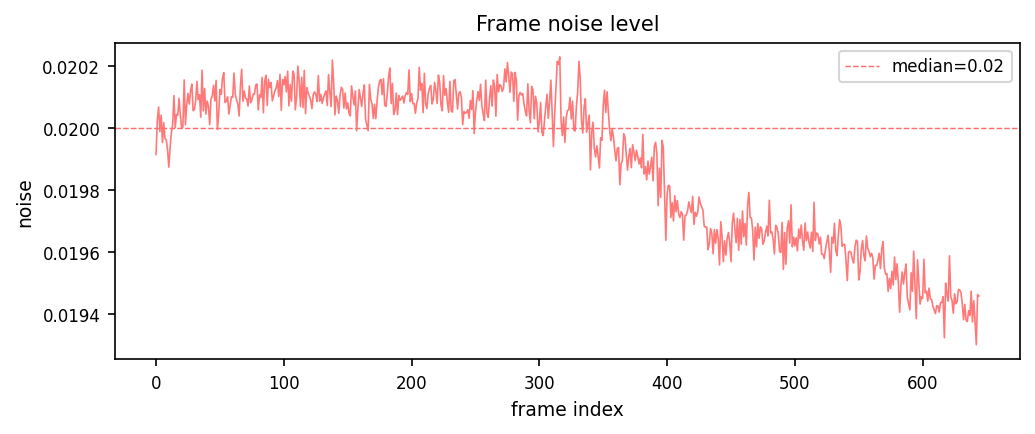
\includegraphics[width=\linewidth]{global_noise.png}
    \caption{Global noise trajectory.}
  \end{subfigure}
  \hfill
  \begin{subfigure}[t]{0.31\textwidth}
    \centering
    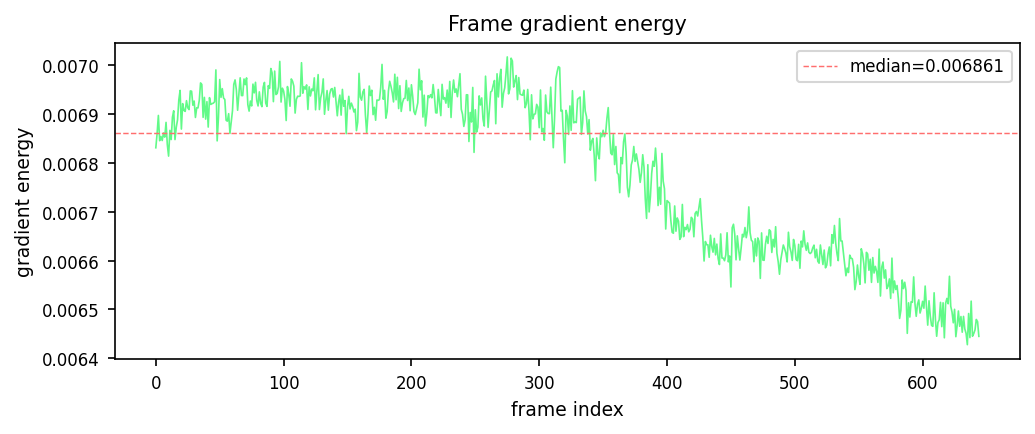
\includegraphics[width=\linewidth]{global_gradient.png}
    \caption{Global gradient-energy trajectory.}
  \end{subfigure}

  \vspace{0.45em}

  \begin{subfigure}[t]{0.31\textwidth}
    \centering
    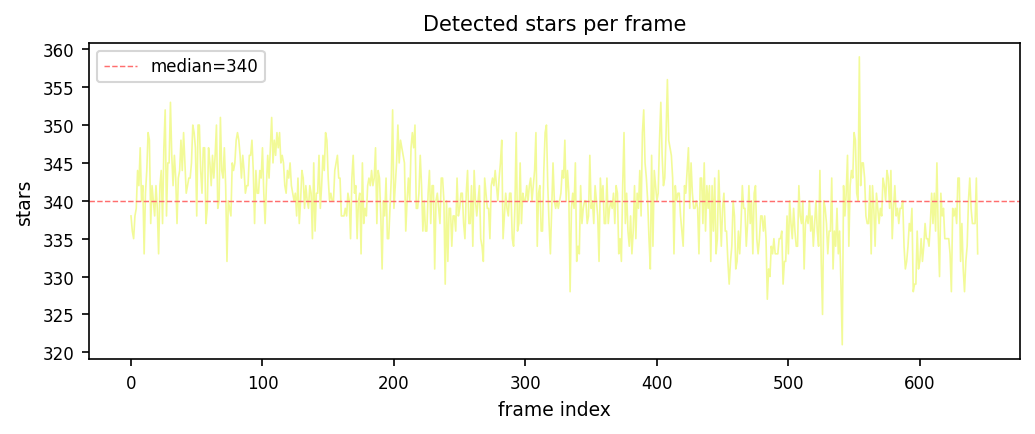
\includegraphics[width=\linewidth]{global_star_count.png}
    \caption{Detected star count per frame.}
  \end{subfigure}
  \hfill
  \begin{subfigure}[t]{0.31\textwidth}
    \centering
    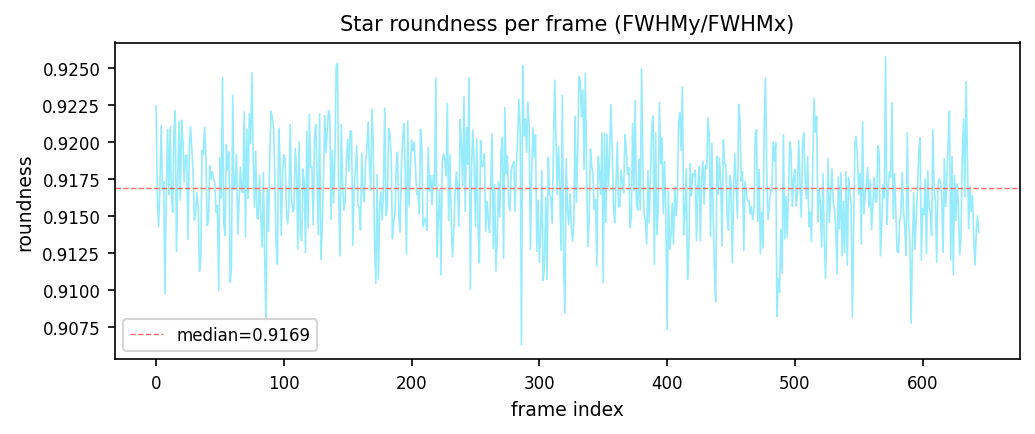
\includegraphics[width=\linewidth]{global_roundness.png}
    \caption{Global roundness trend.}
  \end{subfigure}
  \hfill
  \begin{subfigure}[t]{0.31\textwidth}
    \centering
    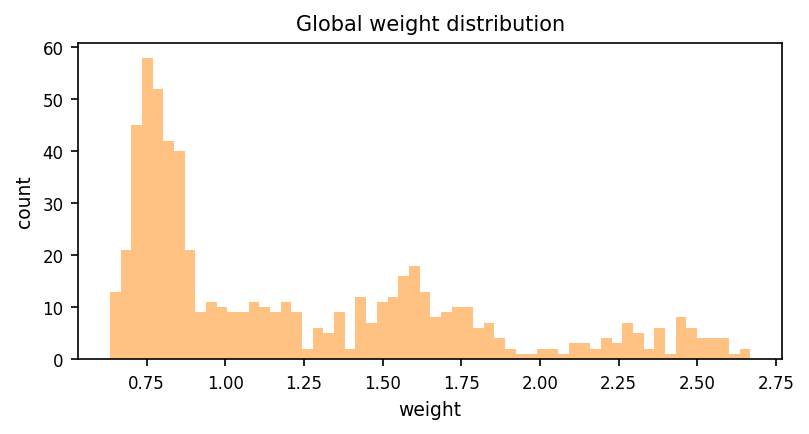
\includegraphics[width=\linewidth]{global_weight_hist.png}
    \caption{Histogram of global reconstruction weights.}
  \end{subfigure}

  \vspace{0.45em}

  \begin{subfigure}[t]{0.31\textwidth}
    \centering
    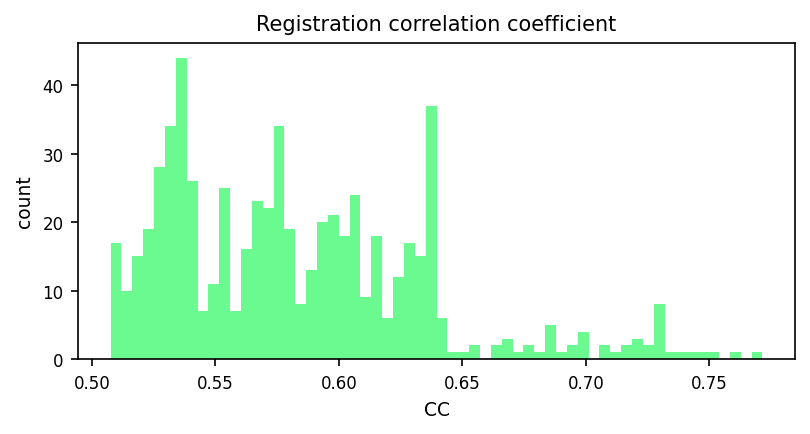
\includegraphics[width=\linewidth]{registration_cc_hist.png}
    \caption{Registration cross-correlation histogram.}
  \end{subfigure}
  \hfill
  \begin{subfigure}[t]{0.31\textwidth}
    \centering
    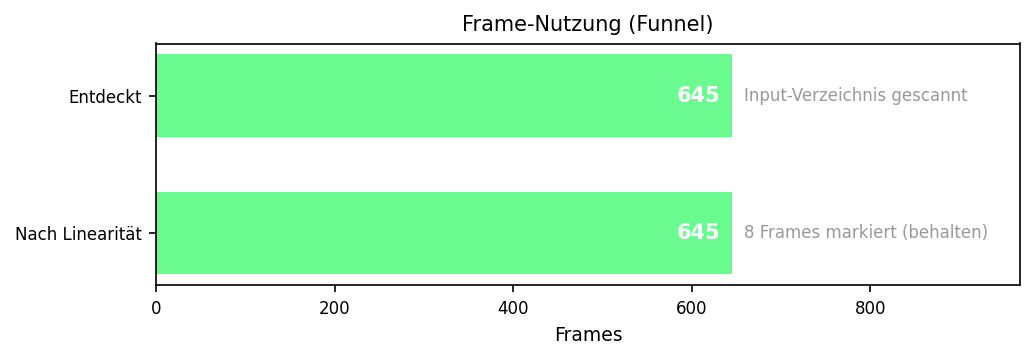
\includegraphics[width=\linewidth]{frame_usage_funnel.png}
    \caption{Frame usage funnel through the pipeline.}
  \end{subfigure}
  \hfill
  \begin{subfigure}[t]{0.31\textwidth}
    \centering
    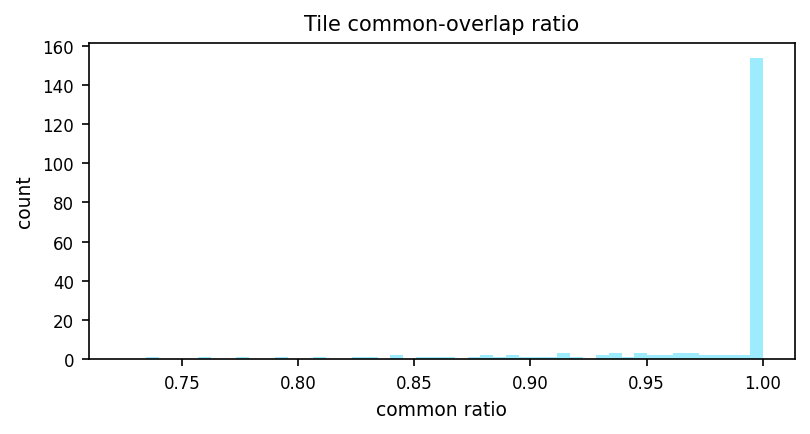
\includegraphics[width=\linewidth]{common_overlap_ratio_hist.png}
    \caption{Common-overlap ratio histogram.}
  \end{subfigure}

  \caption{Compact statistical overview for the M31 run. The nine panels summarize frame-wise background, noise, gradient energy, source detectability, roundness, overlap stability, global weight distribution, registration correlation, and frame-flow behavior.}
  \label{fig:stats_overview}
\end{figure*}

\noindent
The generated diagnostic artifacts add a second layer of interpretation that is more directly tied to the internal state of the reconstruction. Common-overlap diagnostics show that the global shared support remains high, with a canvas-wide common fraction of \num{0.9630}, a median tile overlap ratio of \num{1.000}, and a minimum local ratio of \num{0.6649} at the outer field boundary. This is important because the overlap mask constrains where local quality estimates are physically comparable across the full frame stack.

\noindent
State-clustering diagnostics further show that the dataset separates into 12 synthetic atmospheric states over the feature vector \texttt{(global\_weight, mean\_local\_quality, var\_local\_quality, background, noise)}. Cluster sizes range from 34 to 79 frames with a median of 49.5 frames, which is large enough to support tile-weighted synthetic-frame formation without collapsing into a small number of dominant states.

\begin{figure*}[!t]
  \centering
  \begin{subfigure}[t]{0.31\textwidth}
    \centering
    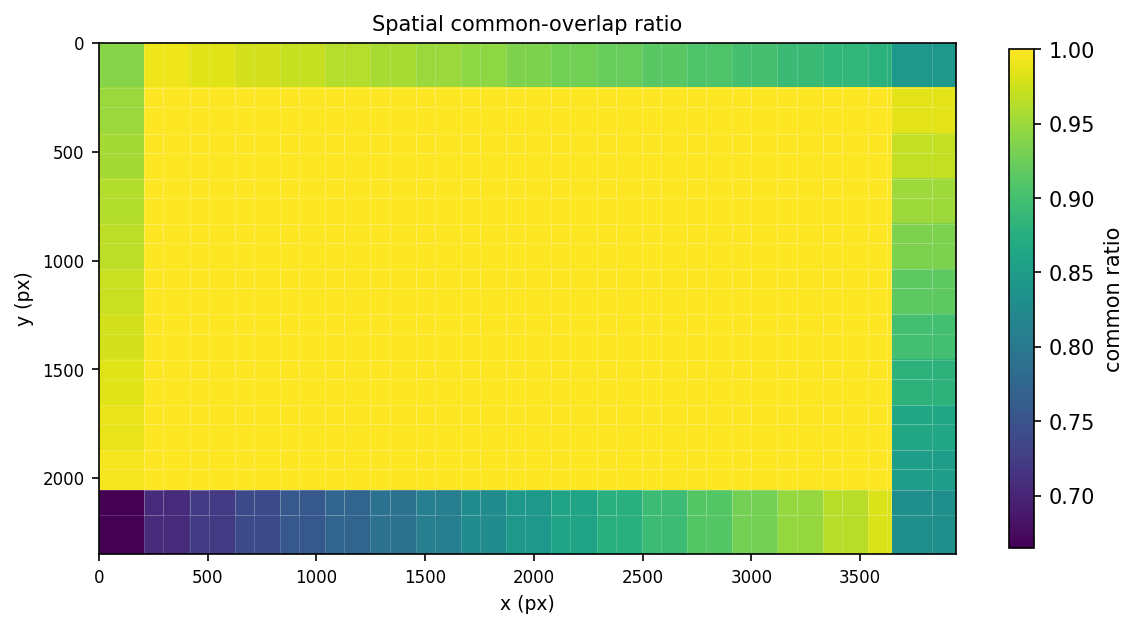
\includegraphics[width=\linewidth]{art_common_overlap_ratio_spatial.png}
    \caption{Spatial map of common-overlap ratio.}
  \end{subfigure}
  \hfill
  \begin{subfigure}[t]{0.31\textwidth}
    \centering
    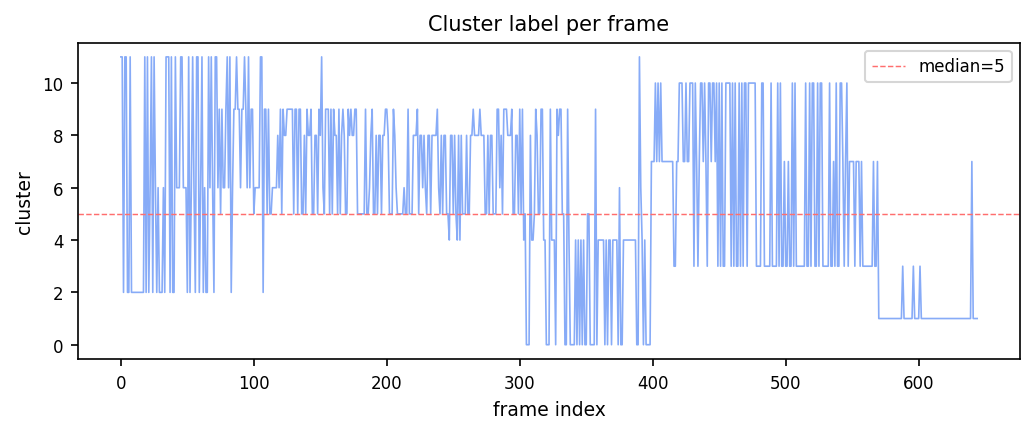
\includegraphics[width=\linewidth]{art_clustering_labels.png}
    \caption{Temporal clustering labels across the frame sequence.}
  \end{subfigure}
  \hfill
  \begin{subfigure}[t]{0.31\textwidth}
    \centering
    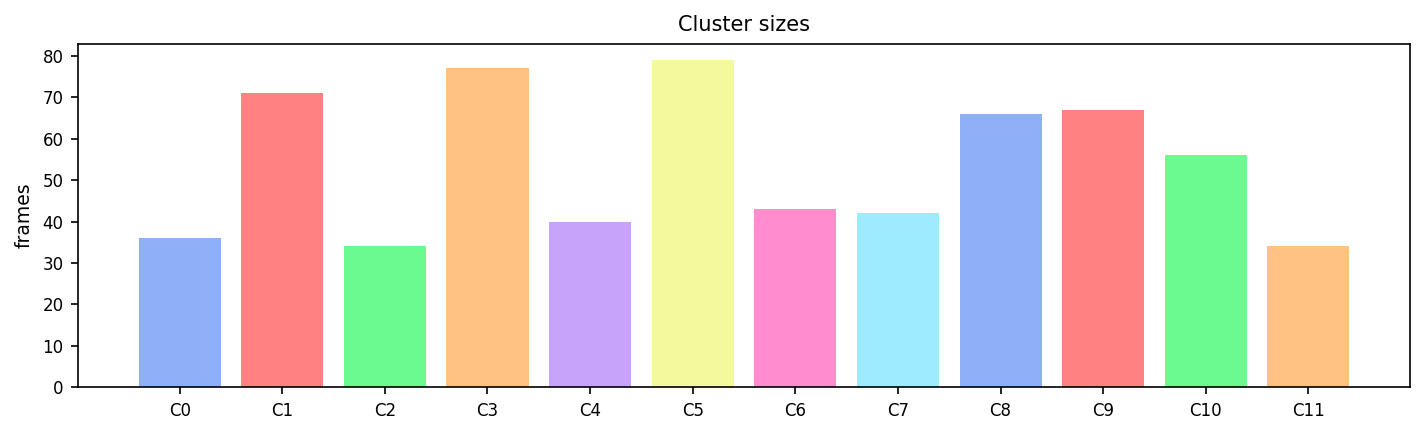
\includegraphics[width=\linewidth]{art_clustering_sizes.png}
    \caption{Cluster-size distribution for the synthetic states.}
  \end{subfigure}

  \vspace{0.45em}

  \begin{subfigure}[t]{0.31\textwidth}
    \centering
    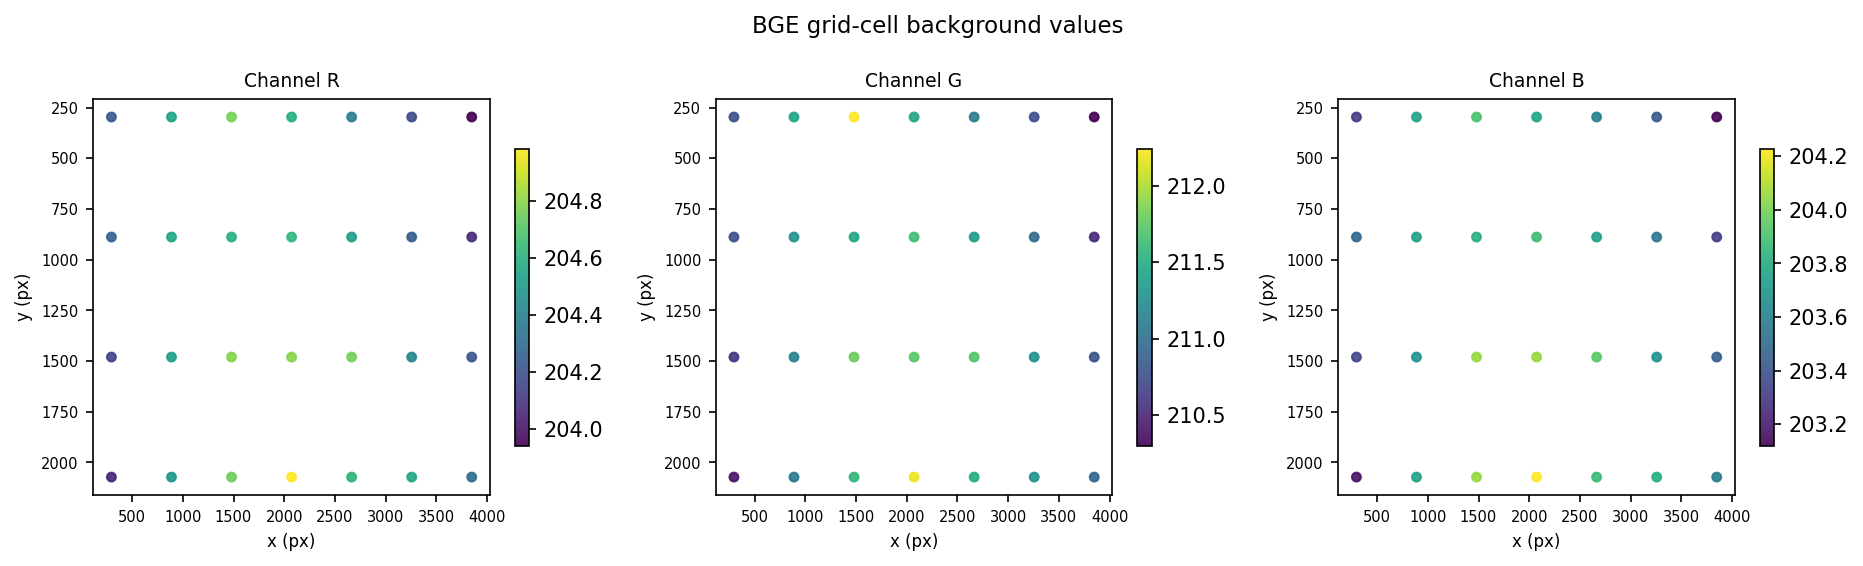
\includegraphics[width=\linewidth]{art_bge_grid_cells.png}
    \caption{BGE coarse-grid cells used for surface fitting.}
  \end{subfigure}
  \hfill
  \begin{subfigure}[t]{0.31\textwidth}
    \centering
    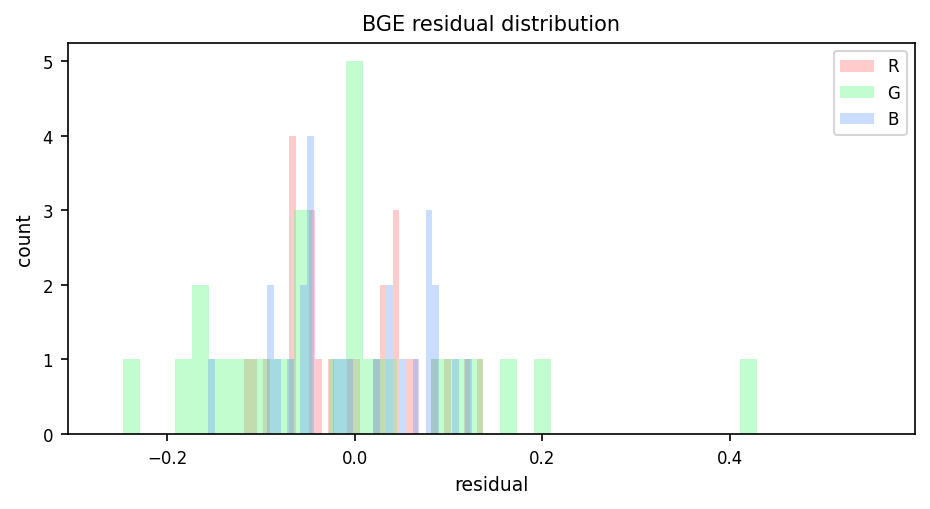
\includegraphics[width=\linewidth]{art_bge_residual_hist.png}
    \caption{Residual histogram of the fitted BGE surface.}
  \end{subfigure}
  \hfill
  \begin{subfigure}[t]{0.31\textwidth}
    \centering
    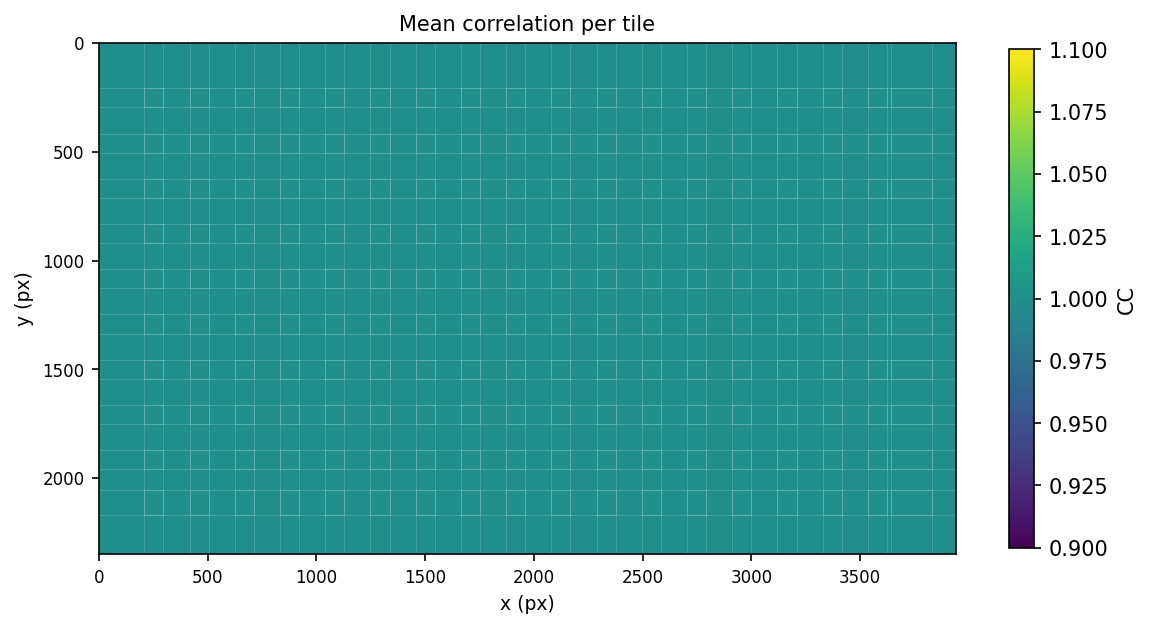
\includegraphics[width=\linewidth]{art_recon_cc_spatial.png}
    \caption{Spatial correlation structure of reconstructed tiles.}
  \end{subfigure}

  \vspace{0.45em}

  \begin{subfigure}[t]{0.48\textwidth}
    \centering
    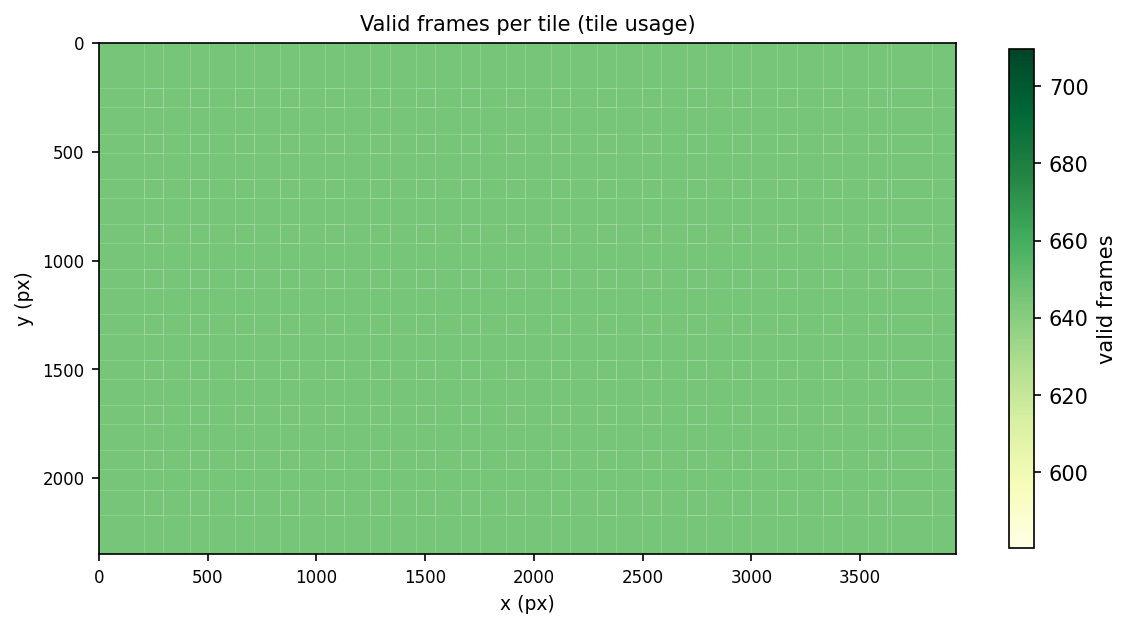
\includegraphics[width=\linewidth]{art_recon_valid_counts_spatial.png}
    \caption{Spatial distribution of valid frame counts contributing to reconstruction.}
  \end{subfigure}
  \caption{Technical diagnostics from the example run. The overlap maps characterize geometric support, the clustering plots visualize how the temporal state model partitions the sequence, and the BGE/reconstruction diagnostics expose whether the downstream background fit and tile-wise accumulation remain spatially stable. In this run, BGE auto-tuning selects a conservative polynomial fit with objective \num{0.09129}; all three channels use 28 valid coarse-grid cells, and the fitted residual RMS is \num{0.0796} (R), \num{0.1836} (G), and \num{0.0823} (B).}
  \label{fig:art_generated_diagnostics}
\end{figure*}

\noindent
The reconstruction-side diagnostics are consistent with the validation summary. No tile fallback is triggered in any of the 209 tiles, tile-weight variance remains at \num{0.2578}, and the measured FWHM improvement is \num{60.394}\% from \num{12.3455} px median seeing to \num{4.8896} px output FWHM. Taken together, these diagnostics show that the method is not only producing a visually plausible final image; it is also maintaining internally coherent overlap support, state partitioning, additive background modeling, and local reconstruction coverage.

\end{document}
